\documentclass[12pt]{article}

\usepackage[margin=1in]{geometry}
\usepackage{times}
\usepackage{booktabs}
\usepackage{xcolor}
\usepackage{setspace}
\usepackage{multicol}
\usepackage{multirow}
\usepackage{threeparttable} 
\usepackage{array}
\usepackage{amsmath}
\usepackage{natbib}
\usepackage{hyperref}
\usepackage{float}
\usepackage{graphicx}
\usepackage[T1]{fontenc}
\usepackage[utf8]{inputenc}

\setlength{\parindent}{0pt}
\setlength{\parskip}{6pt}

\begin{document}

% ===================== TITLE =====================
{\LARGE \textbf{Misalignment, Hubungan Jangka Panjang,\\[0.3cm]
dan Volatilitas Nilai Tukar Riil\\[0.3cm]
Rupiah--Dolar Singapura Periode 2005--2025}}\\[1.2cm]

{\large \textbf{Andreas Syaloom Kurniawan}$^{a}$}\\[0.1cm]
{\small 24/552751/PEK/31194}\\[0.4cm]
{\large \textbf{Ferdinan Adrianus Silalahi}$^{a}$}\\[0.1cm]
{\small 24/551895/PEK/30878}\\[0.7cm]

{\small
$^{a}$\textit{Faculty of Economics and Business, Universitas Gadjah Mada,\\
Jalan Sosio Humaniora No.\ 1, Bulaksumur, Caturtunggal, Depok,\\
Sleman Regency, Special Region of Yogyakarta 55281, Indonesia}\\[0.2cm]
\textit{Email: \href{mailto:andreassyaloomkurniawan@mail.ugm.ac.id}{andreassyaloomkurniawan@mail.ugm.ac.id};
\href{mailto:ferdinanadrianussilalahi@mail.ugm.ac.id}{ferdinanadrianussilalahi@mail.ugm.ac.id}}
}\\[0.8cm]

\hrule
\vspace{0.8cm}

\begin{minipage}[t]{0.28\textwidth}
\raggedright
\textbf{A R T I C L E \quad I N F O}\\[0.3cm]
\hrule
\vspace{0.3cm}
\textbf{JEL classification:}\\[0.15cm]
F31\\
F41\\
O53\\[0.4cm]
\textbf{Keywords:}\\[0.15cm]
Real exchange rate\\
Competitiveness\\
Indonesia\\
Singapore\\
International trade
\end{minipage}
\hfill
\begin{minipage}[t]{0.66\textwidth}
\raggedright
\textbf{A B S T R A C T}\\[0.3cm]
\hrule
\vspace{0.3cm}
Studi ini menganalisis dinamika nilai tukar riil (RER) antara Rupiah Indonesia (IDR) 
dan Dolar Singapura (SGD) selama periode 2005--2025. Dengan menggunakan HP Filter 
untuk mengestimasi RER ekuilibrium dan pendekatan kointegrasi Engle-Granger serta 
Johansen untuk menguji Purchasing Power Parity (PPP), hasil penelitian menunjukkan 
bahwa RER IDR/SGD mengalami misalignment yang bersifat siklikal dengan episode 
undervaluation yang terkonsentrasi pada periode krisis keuangan global 2008--2009 
dan penurunan harga komoditas 2013--2016. Uji kointegrasi mengkonfirmasi adanya 
hubungan keseimbangan jangka panjang antar ketiga variabel, mendukung berlakunya 
\textit{weak PPP} dalam hubungan bilateral Indonesia--Singapura. Namun demikian, 
\textit{strict PPP} ditolak, mengindikasikan bahwa penyesuaian nilai tukar terhadap 
diferensial inflasi bersifat parsial --- konsisten dengan adanya faktor struktural 
seperti efek Balassa-Samuelson dan intervensi kebijakan moneter Bank Indonesia.
\end{minipage}

\vspace{0.8cm}


\section{Introduction}

Real Exchange Rate (RER) merupakan indikator fundamental dalam mengukur daya saing ekonomi suatu negara. Berbeda dengan nilai tukar nominal yang hanya mencerminkan harga relatif mata uang, RER mengakomodasi perbedaan tingkat harga antarnegara, sehingga memberikan gambaran yang lebih akurat tentang posisi kompetitif ekonomi domestik di pasar internasional.

Indonesia sebagai ekonomi terbuka dengan ketergantungan signifikan pada perdagangan internasional menghadapi tantangan dalam menjaga stabilitas nilai tukar riil. Fluktuasi RER tidak hanya berdampak pada daya saing ekspor, tetapi juga berimplikasi pada inflasi domestik, aliran modal, dan kebijakan moneter Bank Indonesia.

Pemahaman mendalam tentang dinamika RER menjadi krusial dalam konteks beberapa pertanyaan ekonomi penting:
\begin{enumerate}
    \item Apakah nilai tukar rupiah saat ini berada pada level ekuilibrium atau mengalami \textit{misalignment}?
    \item Bagaimana hubungan jangka panjang antara nilai tukar nominal dan diferensial inflasi (pengujian Purchasing Power Parity)?
    \item Seberapa volatil RER Indonesia dan apa implikasinya terhadap kebijakan ekonomi?
\end{enumerate}

Penelitian ini bertujuan mengisi gap tersebut dengan pendekatan ekonometrika komprehensif yang menggabungkan analisis stasioneritas, kointegrasi, dan volatilitas RER Indonesia.
\section{Literature Review}
\subsection{Konsep Real Exchange Rate}

Real Exchange Rate (RER) didefinisikan sebagai nilai tukar yang telah disesuaikan dengan perbedaan tingkat harga antarnegara. Secara formal, RER dinyatakan sebagai:

\begin{equation}
    RER = E \times \frac{P^*}{P}
\end{equation}

dimana:
\begin{itemize}
    \item $E$ = nilai tukar nominal (misalnya USD/IDR)
    \item $P^*$ = indeks harga luar negeri (CPI negara mitra dagang)
    \item $P$ = indeks harga domestik (CPI Indonesia)
\end{itemize}

Dalam praktik ekonometrika, transformasi logaritma natural digunakan untuk mempermudah interpretasi elastisitas dan mengurangi heteroskedastisitas:

\begin{equation}
    \ln(RER) = \ln(E) + \ln(P^*) - \ln(P)
\end{equation}

\subsection{Real Effective Exchange Rate (REER)}

Untuk ekonomi dengan multiple trading partners, REER memberikan ukuran agregat yang lebih representatif:

\begin{equation}
    REER = \sum_{i=1}^{n} w_i \times RER_i
\end{equation}

dimana $w_i$ adalah bobot perdagangan dengan negara $i$, dan $\sum w_i = 1$.



\section{Data}

Penelitian ini menggunakan data bulanan periode 2005--2025 yang mencakup
nilai tukar nominal USD/IDR dan SGD/IDR, Consumer Price Index (CPI)
Indonesia, Amerika Serikat, dan Singapura, serta beberapa variabel kontrol
seperti suku bunga, cadangan devisa, dan neraca perdagangan.
Data diperoleh dari dataset yang diberikan dosen metodologi penelitian 
Dr.\ Bagus Santoso, S.E., M.Soc.Sc. Source code dari penugasan ini 
dapat dilihat pada \url{https://github.com/ansyaku/2026-Metolit_ugm/}.
\section{Analisis}

\subsection{Misalignment Analysis}
Sebelum melakukan misalignment analysis, kami kami melakukan transformasi terhadap variabel-variabel, antara lain:
\begin{enumerate}
    \item Mengkonstruksi variabel baru yakni: $\texttt{SGDIDR}$ yang merupakan hasil dari rekalkulasi nilai tukar USD/IDR dengan nilai tukar SGD/USD, dengan cara:
    \begin{equation}
        \texttt{SGDIDR}=\frac{\texttt{USD/IDR}}{\texttt{SGD/USD}}
    \end{equation}
    \item Mentransformasi ke dalam bentuk log \texttt{cpi\_ino}, \texttt{cpi\_sin}.
    \item Konstruksi REER bilateral (Indonesia-US, Indonesia-Singapura)

\end{enumerate}
\begin{figure}
    \centering
    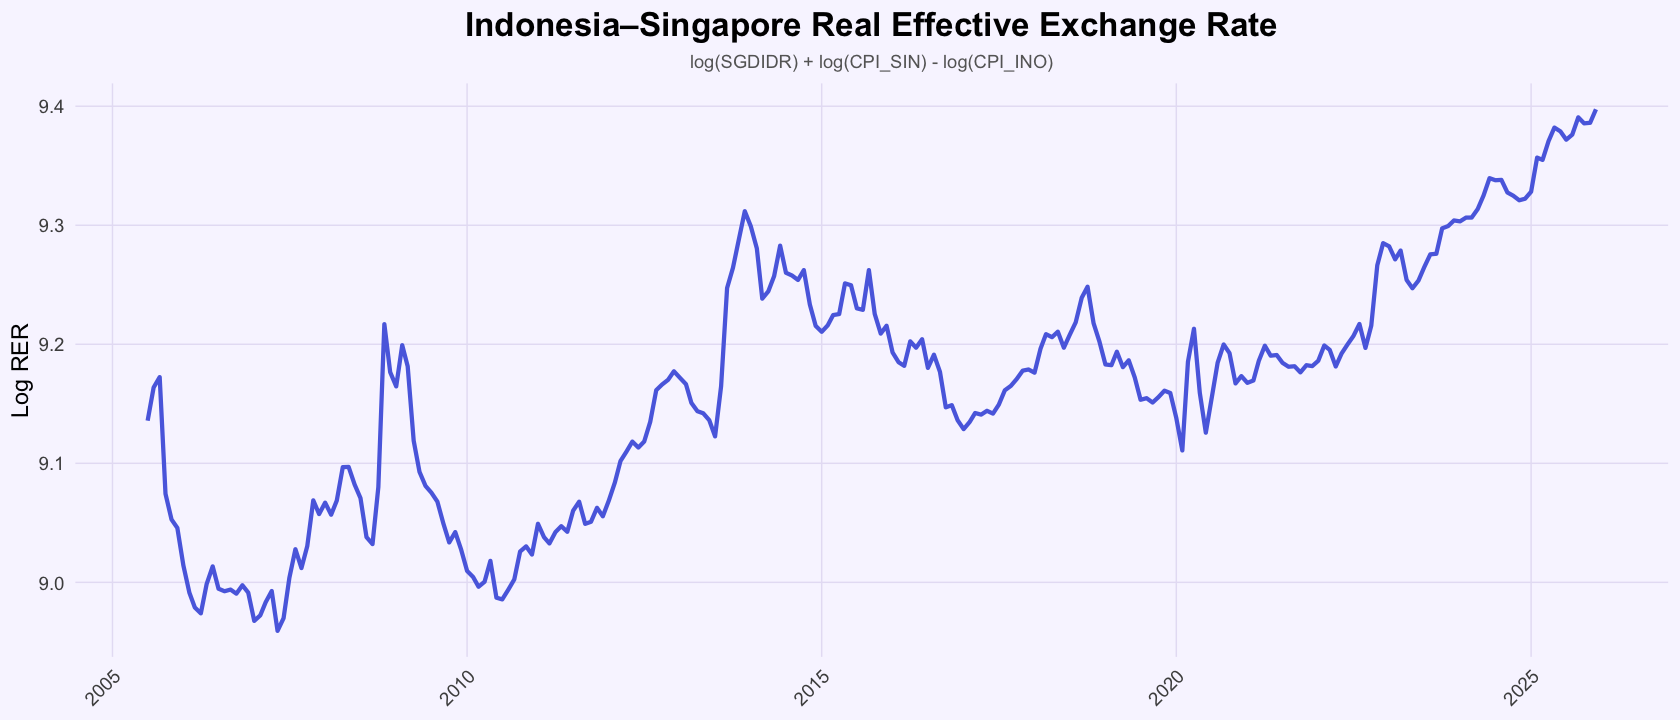
\includegraphics[width=1\linewidth]{SGDIDR_RER.png}
    \caption{RER Dolar Singapura vs Indonesian Rupiahs}
    \label{fig:placeholder}
\end{figure}
Setelah, data dan kurva dari REER dihasilkan, kami selanjutkan menggunakan HP Filter (Hodrick–Prescott filter) untuk menemukan REER Equilibrium. HP Filter merupakan metode statistik dalam time series yang digunakan untuk memisahkan suatu data menjadi komponen trend jangka panjang dan komponen siklus/cycle (fluktuasi sementara), secara ringkas dapat ditulis menjadi:

\[
y_t = \tau_t + c_t
\]

dengan:

\begin{itemize}
    \item $y_t$ = data aktual
    \item $\tau_t$ = komponen trend jangka panjang
    \item $c_t$ = komponen siklus/\textit{cycle} (fluktuasi sementara)
\end{itemize}

Secara algoritmik, HP filter mencari $\tau_t$ yang meminimumkan:

\[
\min_{\{\tau_t\}}
\left[
\underbrace{
\sum_{t=1}^{T} (y_t - \tau_t)^2
}_{\text{goodness of fit}}
+
\lambda
\underbrace{
\sum_{t=2}^{T-1}
\left[
(\tau_{t+1} - \tau_t)
-
(\tau_t - \tau_{t-1})
\right]^2
}_{\text{smoothness penalty}}
\right]
\]

Parameter $\lambda$ mengontrol trade-off antara goodness of fit dan smoothness penalty. Adapun konvensi standar untuk \textbf{data bulanan} $\lambda$ adalah $\lambda = 14400$.

Berdasarkan pengujian dengan menggunakan HP Filter kami mendapati sebagai berikut :
\begin{figure}
    \centering
    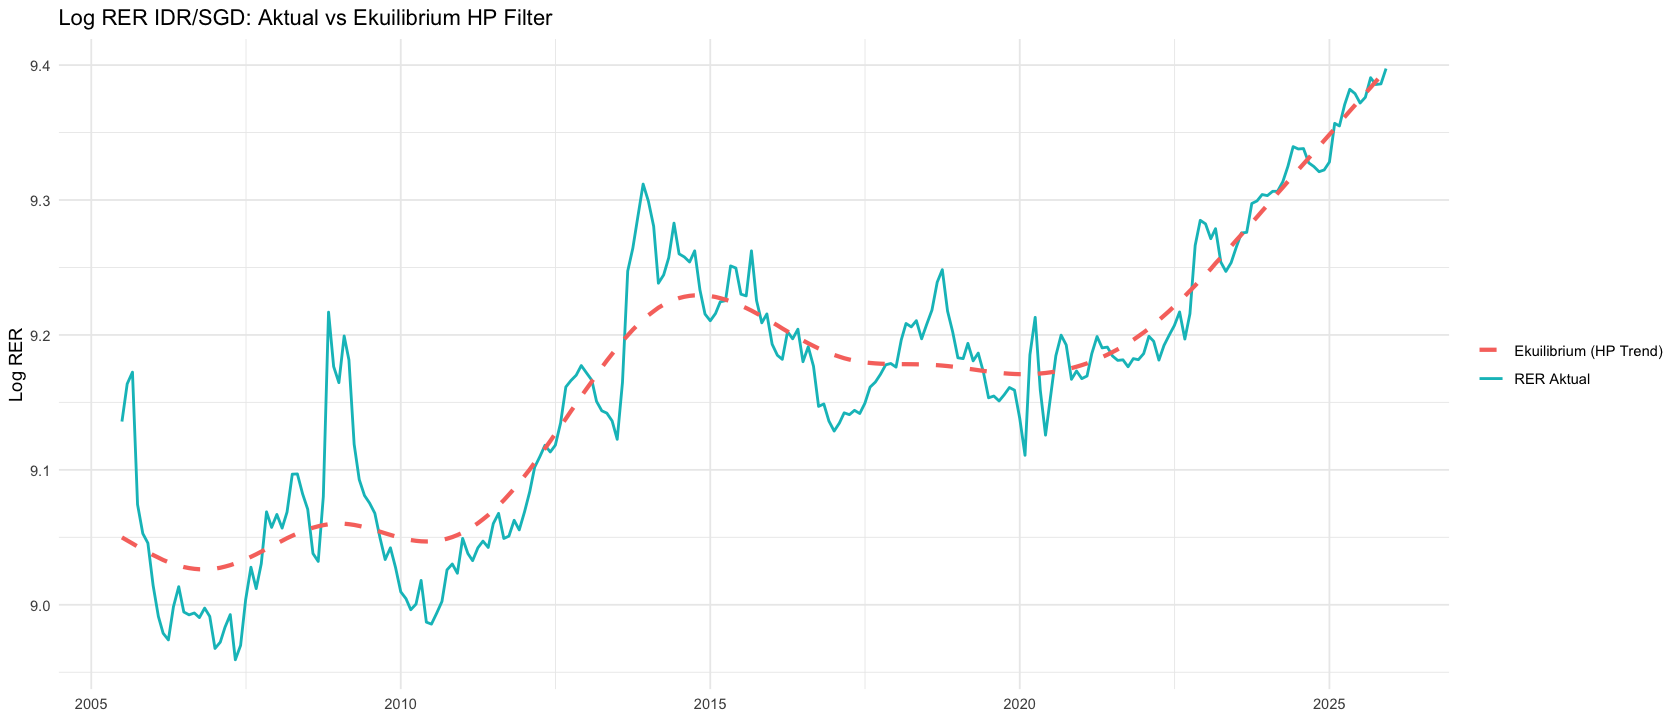
\includegraphics[width=1\linewidth]{HPFilter.png}
    \caption{REER Actual vs REER Equilibrium}
    \label{fig:placeholder}
\end{figure}

Selanjutnya, untuk memudahkan interpretasi, jarak antara REER actual dan REER Ekuilibrium (HP Filter) dapat kita konversi menjadi persentase yang dihitung sebagai:

\begin{equation}
    MISALIGNMENT_t = \frac{REER_t^{actual} - REER_t^{equilibrium}}{REER_t^{equilibrium}} \times 100\%
\end{equation}

\begin{figure}[H]
    \centering
    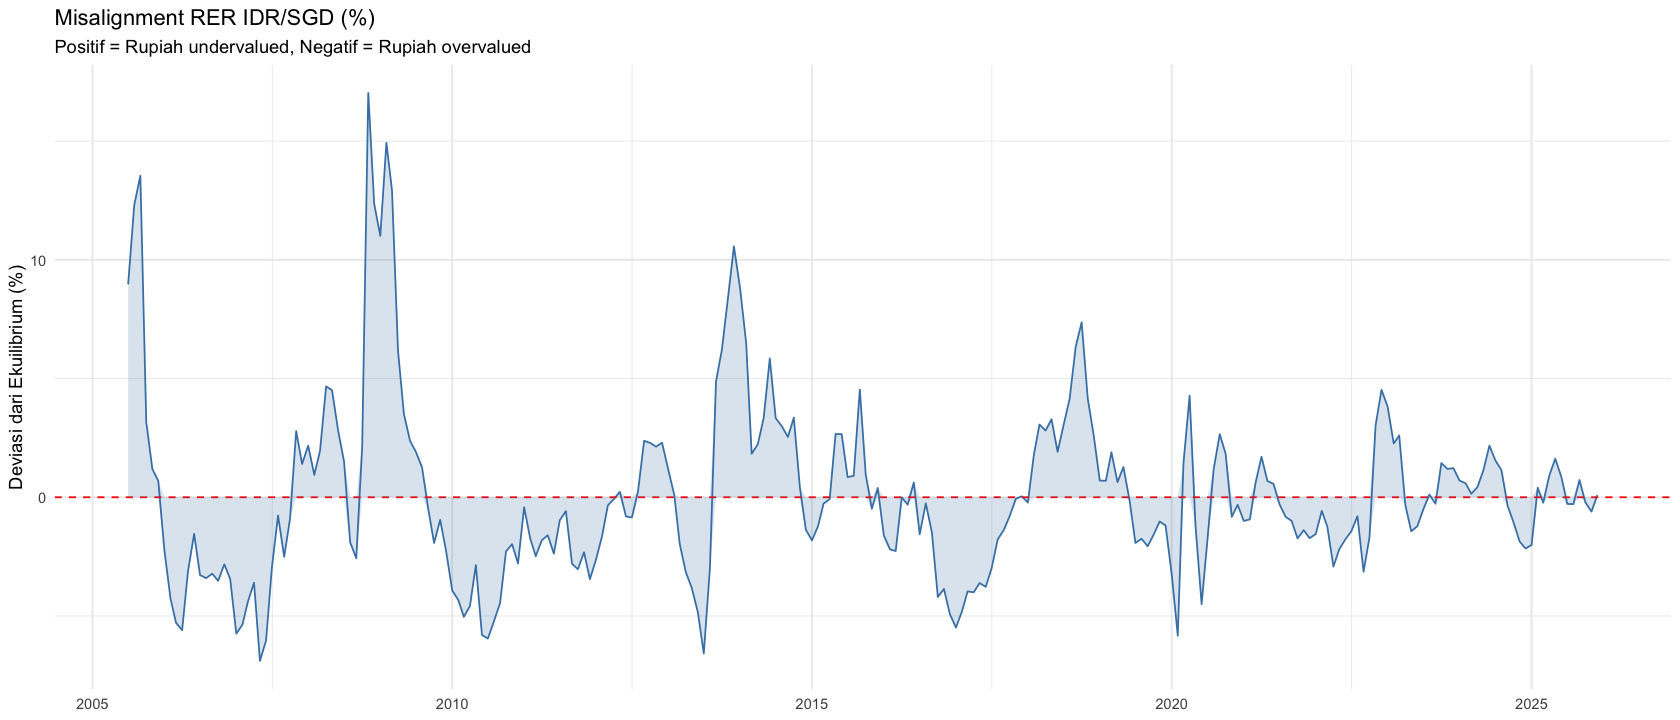
\includegraphics[width=1\linewidth]{Deviasi.png}
    \caption{Penyimpangan REER SGD IDR  Terhadap Ekuilibrium}
    \label{fig:placeholder}
\end{figure}
Dari kedua grafik tersebut dapat kita lihat bahwa, tren jangka panjang \texttt{log RER} naik dari $~9.0 (2005)$ ke $~9.4 (2025)$, artinya Rupiah melemah secara riil terhadap SGD secara struktural sepanjang 20 tahun. Ini konsisten dengan fakta bahwa inflasi Indonesia secara historis lebih tinggi dari Singapura, yang tidak sepenuhnya dikompensasi oleh depresiasi nominal.

Selain itu, kita juga bisa melihat adanya tiga episode misalignment yang terlihat jelas, antara lain :
\begin{enumerate}
    \item \textbf{Periode 2008–2009 (GFC)} \\ 
    RER aktual melonjak tajam di atas ekuilibrium → Rupiah undervalued ekstrem, kemungkinan driven oleh capital flight dan depresiasi nominal yang berlebihan.
\item \textbf{Periode 2013–2016 (Taper Tantrum + commodity bust)}\\
Episode paling panjang RER aktual jauh di atas trend, terlihat Rupiah undervalued persisten, sesuai dengan periode tekanan neraca pembayaran Indonesia saat harga komoditas jatuh.
\item \textbf{Periode 2019–2023}\\ RER aktual konsisten di bawah ekuilibrium, artinya rupiah cenderung overvalued secara riil, mungkin karena capital inflow periode low interest rate global.
\end{enumerate}








\subsection{Long Run Relationship Analysis}

Purchasing Power Parity (PPP) menyatakan bahwa apabila tingkat harga di Indonesia meningkat 
relatif terhadap Singapura, nilai tukar nominal harus menyesuaikan secara proporsional agar 
daya beli riil tetap setara. Dengan demikian, dalam jangka panjang, ketiga variabel 
$\ln(E_t)$, $\ln(P_t)$, dan $\ln(P^*_t)$ tidak dapat bergerak secara independen, harus terdapat 
mekanisme koreksi ekuilibrium yang mengikat ketiganya. 

Berdasarkan definisi Real Exchange Rate (RER):

\begin{equation}
    \ln(\text{RER}_t) = \ln(E_t) + \ln(P^*_t) - \ln(P_t)
\end{equation}

Persamaan kointegrasi yang diestimasi adalah:

\begin{equation}
    \underbrace{\ln(\text{SGDIDR}_t)}_{\ln(E_t)} = \alpha + \beta_1 \underbrace{\ln(\text{CPI\_INO}_t)}_{\ln(P_t)} + \beta_2 \underbrace{\ln(\text{CPI\_SIN}_t)}_{\ln(P^*_t)} + u_t
\end{equation}

\noindent dimana :



\begin{table}[H]
    \centering
    \caption{Variabel dalam Sistem Kointegrasi}
    \begin{tabular}{llll}
        \toprule
        Variabel & Peran & Notasi & Kolom Data \\
        \midrule
        Nilai tukar nominal SGD/IDR & Dependen  & $\ln(E_t)$    & \texttt{log\_SGDIDR} \\
        CPI Indonesia               & Harga domestik & $\ln(P_t)$    & \texttt{log\_cpi\_ino} \\
        CPI Singapura               & Harga luar negeri & $\ln(P^*_t)$  & \texttt{log\_cpi\_sin} \\
        \bottomrule
    \end{tabular}
\end{table}
PPP \textit{ketat} (strict PPP) berlaku apabila estimasi koefisien memenuhi:

\begin{equation}
    \beta_1 = -1 \quad \text{dan} \quad \beta_2 = +1
\end{equation}

Pengujian dilakukan dalam dua langkah:

\begin{enumerate}
    \item \textbf{Unit Root Test} \\
    Estimasi hubungan jangka panjang antara variabel-variabel makroekonomi tidak dapat dilakukan 
    secara langsung melalui regresi OLS apabila sifat stokastik dari masing-masing variabel belum 
    diverifikasi. \citet{Granger1974} menunjukkan bahwa regresi antara dua variabel yang sama-sama 
    non-stasioner $I(1)$ dapat menghasilkan $R^2$ yang tinggi dan koefisien yang tampak signifikan 
    secara statistik, meskipun tidak terdapat hubungan ekonomi apapun di antara keduanya ---
    fenomena yang dikenal sebagai \textit{spurious regression}. Oleh karena itu, sifat stokastik 
    masing-masing variabel $\ln(E_t)$, $\ln(P_t)$, dan $\ln(P^*_t)$ harus diidentifikasi terlebih 
    dahulu. Terdapat tiga kemungkinan hasil yang menentukan langkah analisis selanjutnya:

    \begin{enumerate}
        \item \textbf{Seluruh variabel $I(1)$} \\ Kondisi yang diharapkan dan konsisten dengan 
        prediksi teori PPP; analisis dilanjutkan ke langkah 2.

        \item \textbf{Terdapat variabel $I(0)$} \\ Kointegrasi standar tidak dapat diterapkan. 
        Alternatif yang dipertimbangkan adalah \textit{ARDL bounds test} \citep{Pesaran2001}, 
        yang lebih fleksibel karena tidak mensyaratkan keseragaman orde integrasi.

        \item \textbf{Terdapat variabel $I(2)$} \\ Prosedur \textit{first-differencing} perlu 
        dilakukan dua kali; uji Johansen memiliki prosedur khusus untuk sistem campuran 
        $I(1)$/$I(2)$.
    \end{enumerate}

    \item \textbf{Uji Kointegrasi} \\
    Apabila seluruh variabel terkonfirmasi $I(1)$, uji kointegrasi dilakukan dengan dua metode 
    yang saling melengkapi:

    \begin{enumerate}
        \item \textbf{Engle-Granger Two-Step} \citep{Engle1987} \\ Pada tahap pertama, 
        $\ln(\text{SGDIDR}_t)$ diregresikan pada $\ln(\text{CPI\_INO}_t)$ dan 
        $\ln(\text{CPI\_SIN}_t)$ untuk memperoleh residual $\hat{u}_t$. Pada tahap kedua, 
        stasioneritas $\hat{u}_t$ diuji menggunakan ADF. Apabila $\hat{u}_t \sim I(0)$, 
        disimpulkan bahwa ketiga variabel terkointegrasi.

        \item \textbf{Johansen Cointegration Test} \citep{Johansen1991}\\ Rank kointegrasi 
        ditentukan melalui dua statistik uji: \textit{trace statistic} ($\lambda_{\text{trace}}$) 
        dan \textit{maximum eigenvalue statistic} ($\lambda_{\text{max}}$).
    \end{enumerate}

    Apabila ditemukan hubungan kointegrasi, estimasi dilanjutkan dengan \textit{Vector Error 
    Correction Model} (VECM) untuk memisahkan dinamika jangka pendek dari koreksi menuju 
    ekuilibrium jangka panjang. Sebaliknya, apabila tidak ditemukan kointegrasi, digunakan VAR 
    dalam \textit{first differences} yang hanya mengakomodasi hubungan jangka pendek.
\end{enumerate}

\subsubsection{Hasil Unit Root Test}

Sebelum melakukan analisis kointegrasi, seluruh variabel diuji stasioneritas menggunakan 
Augmented Dickey-Fuller (ADF) dengan pemilihan lag otomatis berdasarkan kriteria AIC. 
Spesifikasi \textit{drift} digunakan untuk $\ln(\text{SGDIDR}_t)$ mengingat nilai tukar 
tidak memiliki tren deterministik yang jelas, sementara spesifikasi \textit{trend} digunakan 
untuk $\ln(\text{CPI\_INO}_t)$ dan $\ln(\text{CPI\_SIN}_t)$ karena indeks harga secara 
teoritis mengikuti tren deterministik positif.

\begin{table}[H]
    \centering
    \caption{Hasil Augmented Dickey-Fuller (ADF) Unit Root Test}
    \label{tab:unitroot}
    \begin{tabular}{lcccccc}
        \toprule
        \multirow{2}{*}{Variabel} 
            & \multicolumn{2}{c}{Level} 
            & \multicolumn{2}{c}{First Difference} 
            & \multirow{2}{*}{Kesimpulan} \\
        \cmidrule(lr){2-3} \cmidrule(lr){4-5}
            & $\tau$ & CV 5\% & $\tau$ & CV 5\% & \\
        \midrule
        $\ln(\text{SGDIDR})$  & $-0.731$ & $-2.880$ & $-12.502^{***}$ & $-2.880$ & $I(1)$ \\
        $\ln(\text{CPI\_INO})$ & $-3.291$ & $-3.430$ & $-10.613^{***}$ & $-2.880$ & $I(1)$ \\
        $\ln(\text{CPI\_SIN})$ & $-1.146$ & $-3.430$ & $-12.696^{***}$ & $-2.880$ & $I(1)$ \\
        \bottomrule
    \end{tabular}
    \begin{tablenotes}
        \small
        \item \textit{Catatan:} $^{***}$ signifikan pada taraf 1\%. Hipotesis nol: 
        variabel mengandung unit root. Spesifikasi \textit{drift} untuk 
        $\ln(\text{SGDIDR})$; spesifikasi \textit{trend} untuk variabel CPI pada 
        level. Pemilihan lag menggunakan kriteria AIC.
    \end{tablenotes}
\end{table}
Hasil pengujian pada Tabel~\ref{tab:unitroot} menunjukkan bahwa seluruh variabel gagal 
menolak hipotesis nol pada level — nilai $\tau$ seluruhnya berada di atas \textit{critical 
value} 5\% — mengindikasikan keberadaan unit root. Setelah dilakukan \textit{first 
differencing}, ketiga variabel menjadi stasioner secara signifikan pada taraf 1\%, dengan 
nilai $\tau$ yang jauh melampaui \textit{critical value} ($-12.502$, $-10.613$, dan $-12.696$ 
dibandingkan CV $-2.880$). \\
\textcolor{blue}{Dengan demikian, seluruh variabel terkonfirmasi terintegrasi pada 
orde satu, $I(1)$, sehingga syarat perlu untuk analisis kointegrasi terpenuhi.}

\subsubsection{Hasil Cointegration Test}
\subsubsection*{Engle-Granger Two-Step}
\paragraph{Step 1: Regresi Kointegrasi}
\noindent
Estimasi OLS pada persamaan kointegrasi menghasilkan:

\begin{equation}
    \widehat{\ln(\text{SGDIDR}_t)} = 4.9794 + 0.8519\ln(\text{CPI\_INO}_t) + 0.0923\ln(\text{CPI\_SIN}_t)
\end{equation}

\begin{table}[H]
    \centering
    \caption{Hasil Estimasi Regresi Kointegrasi (Step 1)}
    \label{tab:eg_step1}
    \begin{tabular}{lcccc}
        \toprule
        Variabel & Koefisien & Std. Error & $t$-stat & $p$-value \\
        \midrule
        Konstanta ($\alpha$)           & $4.9794$ & $0.2436$ & $20.439$ & $<0.001^{***}$ \\
        $\ln(\text{CPI\_INO})$ ($\beta_1$) & $0.8519$  & $0.0417$ & $20.427$ & $<0.001^{***}$ \\
        $\ln(\text{CPI\_SIN})$ ($\beta_2$) & $0.0923$  & $0.0930$ & $0.993$  & $0.322$ \\
        \midrule
        \multicolumn{2}{l}{$R^2$}                   & \multicolumn{3}{c}{$0.9561$} \\
        \multicolumn{2}{l}{$\bar{R}^2$}              & \multicolumn{3}{c}{$0.9557$} \\
        \multicolumn{2}{l}{$F$-statistic}            & \multicolumn{3}{c}{$2645$ ($p < 0.001$)} \\
        \multicolumn{2}{l}{Observasi}                & \multicolumn{3}{c}{$246$} \\
        \bottomrule
    \end{tabular}
    \begin{tablenotes}
        \small
        \item \textit{Catatan:} $^{***}$ signifikan pada taraf 1\%. Variabel dependen: 
        $\ln(\text{SGDIDR}_t)$.
    \end{tablenotes}
\end{table}

\paragraph{Step 2: Uji Stasioneritas Residual}
\noindent
Residual $\hat{u}_t$ dari persamaan kointegrasi diuji menggunakan ADF tanpa intercept 
dan trend, sesuai prosedur \citet{Engle1987}. Hasil pengujian disajikan pada 
Tabel~\ref{tab:eg_step2}.

\begin{table}[H]
    \centering
    \caption{ADF Test pada Residual Kointegrasi}
    \label{tab:eg_step2}
    \begin{tabular}{lcccc}
        \toprule
        & $\tau$ & CV 1\% & CV 5\% & CV 10\% \\
        \midrule
        Residual $\hat{u}_t$ & $-4.5645^{***}$ & $-2.580$ & $-1.950$ & $-1.620$ \\
        \bottomrule
    \end{tabular}
    \begin{tablenotes}
        \small
        \item \textit{Catatan:} $^{***}$ menolak hipotesis nol unit root pada taraf 1\%. 
        Spesifikasi tanpa intercept dan trend. Pemilihan lag menggunakan kriteria AIC.
    \end{tablenotes}
\end{table}

Nilai $\tau = -4.5645$ melampaui \textit{critical value} pada taraf 1\% ($-2.580$), 
sehingga hipotesis nol unit root pada residual ditolak secara tegas.\\
\textcolor{blue}{Dengan demikian, 
$\hat{u}_t \sim I(0)$,  disimpulkan bahwa $\ln(\text{SGDIDR}_t)$, 
$\ln(\text{CPI\_INO}_t)$, dan $\ln(\text{CPI\_SIN}_t)$ \textbf{terkointegrasi}, yakni  
terdapat hubungan keseimbangan jangka panjang di antara ketiga variabel.}

\paragraph{Implikasi terhadap PPP}

Meskipun kointegrasi terkonfirmasi, pengujian restriksi PPP ketat menunjukkan bahwa 
koefisien yang diestimasi secara signifikan menyimpang dari nilai teoritis 
$\beta_1 = -1$ dan $\beta_2 = +1$:

\begin{table}[H]
    \centering
    \caption{Uji Restriksi PPP Ketat}
    \label{tab:ppp_test}
    \begin{tabular}{lccccc}
        \toprule
        Hipotesis & $\hat{\beta}$ & Nilai Teoritis & $t$-stat & $p$-value & Keputusan \\
        \midrule
        $H_0: \beta_1 = -1$ & $0.8519$ & $-1$ & $44.405$ & $<0.001$ & Tolak $H_0$ \\
        $H_0: \beta_2 = +1$ & $0.0923$ & $+1$ & $-9.766$ & $<0.001$ & Tolak $H_0$ \\
        \bottomrule
    \end{tabular}
\end{table}

Kedua restriksi ditolak pada taraf 1\%, mengindikasikan bahwa \textbf{PPP ketat tidak 
berlaku} dalam periode sampel. Selain itu, dapat juga diketahui bahwa :
\begin{enumerate}
    \item $\hat{\beta}_1 = 0.8519$ — positif dan signifikan, menunjukkan bahwa kenaikan harga 
domestik Indonesia justru \textit{berkorelasi positif} dengan depresiasi SGD/IDR, 
berlawanan arah dengan prediksi PPP yang mensyaratkan $\beta_1 = -1$.
\item $\hat{\beta}_2 = 0.0923$ tidak signifikan secara statistik ($p = 0.322$), 
mengindikasikan bahwa harga Singapura tidak memiliki pengaruh yang terdeteksi terhadap 
nilai tukar nominal dalam jangka panjang. 
\end{enumerate}


Temuan ini konsisten dengan literatur yang 
mendokumentasikan kegagalan PPP pada horizon jangka menengah untuk negara berkembang 
\citep{Rogoff1996}, dan mengindikasikan adanya faktor struktural lain seperti 
perbedaan produktivitas (efek Balassa-Samuelson) atau rigiditas harga yang 
memediasi hubungan antara diferensial inflasi dan nilai tukar.

\subsubsection{Hasil Johansen Cointegration Test}

Sebagai konfirmasi terhadap hasil Engle-Granger, uji kointegrasi Johansen dilakukan 
pada sistem VAR dengan lag optimal $K = 7$ berdasarkan kriteria AIC. Pengujian 
menggunakan dua statistik yakni \textit{trace statistic} ($\lambda_{\text{trace}}$) dan 
\textit{maximum eigenvalue statistic} ($\lambda_{\text{max}}$), dengan spesifikasi 
konstanta dalam hubungan kointegrasi (\textit{ecdet = "const"}).

\begin{table}[H]
    \centering
    \caption{Johansen Cointegration Test --- Trace Statistic}
    \label{tab:johansen_trace}
    \begin{tabular}{lccccl}
        \toprule
        $H_0$ & $\lambda_{\text{trace}}$ & CV 10\% & CV 5\% & CV 1\% & Keputusan \\
        \midrule
        $r = 0$    & $59.71$ & $32.00$ & $34.91$ & $41.07$ & Tolak $H_0^{***}$ \\
        $r \leq 1$ & $21.31$ & $17.85$ & $19.96$ & $24.60$ & Tolak $H_0^{**}$ \\
        $r \leq 2$ & $4.41$  & $7.52$  & $9.24$  & $12.97$ & Gagal tolak $H_0$ \\
        \bottomrule
    \end{tabular}
    \begin{tablenotes}
        \small
        \item \textit{Catatan:} $^{***}$ dan $^{**}$ menunjukkan penolakan $H_0$ pada 
        taraf 1\% dan 5\%. Lag $K = 7$ dipilih berdasarkan kriteria AIC.
    \end{tablenotes}
\end{table}

\begin{table}[H]
    \centering
    \caption{Johansen Cointegration Test --- Maximum Eigenvalue Statistic}
    \label{tab:johansen_eigen}
    \begin{tabular}{lccccl}
        \toprule
        $H_0$ & $\lambda_{\text{max}}$ & CV 10\% & CV 5\% & CV 1\% & Keputusan \\
        \midrule
        $r = 0$    & $38.40$ & $19.77$ & $22.00$ & $26.81$ & Tolak $H_0^{***}$ \\
        $r \leq 1$ & $16.90$ & $13.75$ & $15.67$ & $20.20$ & Tolak $H_0^{**}$ \\
        $r \leq 2$ & $4.41$  & $7.52$  & $9.24$  & $12.97$ & Gagal tolak $H_0$ \\
        \bottomrule
    \end{tabular}
    \begin{tablenotes}
        \small
        \item \textit{Catatan:} $^{***}$ dan $^{**}$ menunjukkan penolakan $H_0$ pada 
        taraf 1\% dan 5\%.
    \end{tablenotes}
\end{table}

Kedua statistik uji secara konsisten mengindikasikan \textbf{rank kointegrasi $r = 2$}: 
hipotesis $r = 0$ dan $r \leq 1$ ditolak, sementara $r \leq 2$ gagal ditolak bahkan 
pada taraf 10\%. \\
\textcolor{blue}{
Dengan demikian, terdapat dua hubungan kointegrasi yang independen 
dalam sistem, mengkonfirmasi dan memperkuat temuan Engle-Granger.}

Vektor kointegrasi pertama (dinormalisasi pada $\ln(\text{SGDIDR})$) adalah:

\begin{equation}
    \ln(\text{SGDIDR}_t) - 1.2951\ln(\text{CPI\_INO}_t) + 0.2307\ln(\text{CPI\_SIN}_t) 
    = 4.3009
    \label{eq:coint_vec}
\end{equation}

Koefisien $\hat{\beta}_1 = -1.2951$ dan $\hat{\beta}_2 = 0.2307$ kembali menyimpang 
dari restriksi PPP ketat ($\beta_1 = -1$, $\beta_2 = +1$), konsisten dengan temuan 
Engle-Granger. Keberadaan dua vektor kointegrasi ($r = 2$) sendiri merupakan temuan 
yang menarik: dalam sistem tiga variabel $I(1)$, rank kointegrasi maksimum adalah 2, 
yang mengimplikasikan bahwa sistem hampir sepenuhnya terikat oleh hubungan ekuilibrium 
jangka panjang dengan hanya satu \textit{common stochastic trend} yang mendorong 
dinamika bersama ketiga variabel.

\newpage
Tabel~\ref{tab:coint_summary} merangkum hasil kedua metode kointegrasi.

\begin{table}[H]
    \centering
    \caption{Ringkasan Hasil Uji Kointegrasi}
    \label{tab:coint_summary}
    \begin{tabular}{llll}
        \toprule
        Metode & Statistik Uji & Hasil & Kesimpulan \\
        \midrule
        Engle-Granger & $\tau = -4.5645$ & $< $ CV 1\% $(-2.580)$ 
            & Terkointegrasi \\
        Johansen Trace & $\lambda_{\text{trace}} = 59.71$ $(r=0)$ 
            & $>$ CV 1\% $(41.07)$ & $r = 2$ \\
        Johansen Max-$\lambda$ & $\lambda_{\text{max}} = 38.40$ $(r=0)$ 
            & $>$ CV 1\% $(26.81)$ & $r = 2$ \\
        \midrule
        \multicolumn{3}{l}{\textbf{Kesimpulan keseluruhan}} 
            & \textbf{PPP lemah berlaku} \\
        \bottomrule
    \end{tabular}
    \begin{tablenotes}
        \small
        \item \textit{Catatan:} Kedua metode konsisten mengkonfirmasi adanya hubungan 
        kointegrasi. PPP ketat ditolak berdasarkan uji restriksi koefisien; namun 
        hubungan jangka panjang antara nilai tukar nominal dan tingkat harga bilateral 
        terkonfirmasi, konsisten dengan PPP dalam bentuk lemah.
    \end{tablenotes}
\end{table}

Secara keseluruhan, \textcolor{blue}{hasil uji kointegrasi dengan dua metode yang saling melengkapi 
(Engle-Granger dan Johansen) secara konsisten mengkonfirmasi adanya hubungan 
keseimbangan jangka panjang antara nilai tukar nominal SGD/IDR, tingkat harga 
domestik Indonesia, dan tingkat harga Singapura}. 
\begin{itemize}
    \item Temuan ini \textbf{mendukung berlakunya 
\textit{weak PPP}} dalam hubungan bilateral Indonesia-Singapura: ketiga variabel 
terikat oleh mekanisme ekuilibrium jangka panjang yang mencegah penyimpangan 
permanen, sebagaimana dibuktikan oleh stasioneritas residual kointegrasi 
($\tau = -4.5645$, signifikan pada taraf 1\%) dan rank kointegrasi $r = 2$ pada 
uji Johansen. 
\item Namun demikian, \textbf{\textit{strict PPP} ditolak secara tegas}, hal ini terlihat dari koefisien 
yang diestimasi ($\hat{\beta}_1 = 0.8519$, $\hat{\beta}_2 = 0.0923$) menyimpang 
signifikan dari restriksi teoritis $\beta_1 = -1$ dan $\beta_2 = +1$ yang 
mengindikasikan bahwa penyesuaian nilai tukar terhadap diferensial inflasi bilateral 
bersifat parsial dan tidak proporsional.
\end{itemize}
 


\newpage
\subsection{Volatility Analysis}
Lorem ipsum dolor sit amet, consectetur adipiscing elit. Pellentesque nibh.


\section{Conclusion}
Lorem ipsum dolor sit amet, consectetur adipiscing elit. Pellentesque nibh.

% ... isi paper ...

\bibliographystyle{apalike}
\bibliography{references}

\end{document}
